%!TEX program = xelatex
% 如果你有参考文献(myref.bib),请按 xelatex -> bibtex -> xelatex*2 的顺序进行编译
\documentclass[dvipsnames, svgnames,a4paper,11pt]{article}
% ----------------------------------------------------
%   中山大学物理与天文学院本科实验报告模板
%   作者:Huanyu Shi,2019级
%   Github:https://github.com/huanyushi/SYSU-SPA-Labreport-Template
%   知乎:https://www.zhihu.com/people/za-ran-zhu-fu-liu-xing
%   Last update : 2024.10.27
% ----------------------------------------------------

\input{settings} % 导入模板的相关设置
\usepackage{lipsum}


%---------------------------------------------------------------------
%	正文
%---------------------------------------------------------------------

\begin{document}

\scoresTable{}{}{}{}{}{}{}{}

% \infoTable{专业}{年级}{姓名}{学号}{实验时间}{教师签名}
\infoTable{物理学}{2019级}{Huanyu Shi}{19342091}{}{}

\begin{center}
	\LARGE Template \quad 实验报告模板
\end{center}

\textbf{【实验报告注意事项】}
\begin{enumerate}
	\item 实验报告由三部分组成:
	\begin{enumerate}
		\item 预习报告:(提前一周)认真研读\underline{\textbf{实验讲义}},弄清实验原理;实验所需的仪器设备、用具及其使用(强烈建议到实验室预习),完成课前预习思考题;了解实验需要测量的物理量,并根据要求提前准备实验记录表格(第一循环实验已由教师提供模板,可以打印)。预习成绩低于10分(共20分)者不能做实验。
	    \item 实验记录:认真、客观记录实验条件、实验过程中的现象以及数据。实验记录请用珠笔或者钢笔书写并签名(\textcolor{red}{\textbf{用铅笔记录的被认为无效}})。\textcolor{red}{\textbf{保持原始记录,包括写错删除部分,如因误记需要修改记录,必须按规范修改。}}(不得输入电脑打印,但可扫描手记后打印扫描件);离开前请实验教师检查记录并签名。
	    \item 分析讨论:处理实验原始数据(学习仪器使用类型的实验除外),对数据的可靠性和合理性进行分析;按规范呈现数据和结果(图、表),包括数据、图表按顺序编号及其引用;分析物理现象(含回答实验思考题,写出问题思考过程,必要时按规范引用数据);最后得出结论。
	\end{enumerate}
	\textbf{实验报告就是将预习报告、实验记录、和数据处理与分析合起来,加上本页封面。}
	\item 每次完成实验后的一周内交\textbf{实验报告}(特殊情况不能超过两周)。
	\item 除实验记录外,实验报告其他部分建议双面打印。
\end{enumerate}


\clearpage
\tableofcontents
\clearpage

\setcounter{section}{0}
\nsection{Template}{光电效应实验}{预习报告}
	
\subsection{实验目的}
\begin{enumerate}
	\item 了解光电效应的规律,加深对光的量子性的理解;
	\item 测量不同光频率下的截止电压,计算普朗克常量$h$,测量光电管的伏安特性。
\end{enumerate}

\subsection{仪器用具}
\begin{table}[htbp]
	\centering
	\renewcommand\arraystretch{1.6}
	% \setlength{\tabcolsep}{10mm}
	\begin{tabular}{p{0.05\textwidth}|p{0.20\textwidth}|p{0.05\textwidth}|p{0.5\textwidth}}
	\hline
	编号& 仪器用具名称 & 数量 &  主要参数(型号,测量范围,测量精度等) \\
	\hline
	1&高压汞灯 &1 & BEM-5005, 50W/220 VAC,谱线:365nm, 405nm, 436nm, 546nm, 577nm\\

	2&光电管 &1 & BEM-5006, 光谱响应范围:300-700 nm,滤光片(中心波长分别为365nm, 405nm, 436nm, 546nm, 577nm),
	光阑(直径分别为2mm, 4mm, 8mm)、遮光盖、线缆等 \\
	
	3&微电流放大器 & 1 &BEM-5004 \\
	
	4&可调直流电源&1 & GPP-4323, 4通道, 32V/3A$\times$2 (CH1/CH2), 5V/1A (CH3), 15V/1A (CH4)\\
	\hline
\end{tabular}
\end{table}

\subsection{原理概述}
\begin{wrapfigure}{l}{0cm} % l 表示靠文字内容的左侧,0cm 表示环境横向长度
	\centering
	
\includegraphics[width=0.3\textwidth]{example.png}
	\caption{环绕图片示例}
\end{wrapfigure}
\textcolor{red}{参考文献示例},参考\cite{test1,test2}。

光电效应(英语:Photoelectric Effect)是指光束照射物体时会使其发射出电子的物理效应。发射出来的电子称为“光电子”。

光束里的光子所拥有的能量与光的频率成正比。假若金属里的电子吸收了一个光子的能量,而这能量大于或等于某个与金属相关的能量阈值(称为这种金属的逸出功),
则此电子因为拥有了足够的能量,会从金属中逃逸出来,成为光电子;若能量不足,则电子会释出能量,能量重新成为光子离开,电子能量恢复到吸收之前,
无法逃逸离开金属。增加光束的辐照度(光束的强度)会增加光束里光子的密度,在同一段时间内激发更多的电子,但不会
使得每一个受激发的电子因吸收更多的光子而获得更多的能量。换言之,光电子的能量与辐照度无关,只与光子的能量、频率有关。

被光束照射到的电子会吸收光子的能量,但是其中机制遵照的是一种非全有即全无的准则,光子所有能量都必须被吸收,用来克服逸出功,
否则这能量会被释出。假若电子所吸收的能量能够克服逸出功,并且还有剩馀能量,则这剩余能量会成为电子在被发射后的动能。

逸出功$W_0$是从金属表面发射出一个光电子所需要的最小能量。如果转换到频率的角度来看,光子的频率必须大于金属特征的极限频率,
才能给予电子足够的能量克服逸出功。逸出功与极限频率$\nu_0$之间的关系为
\begin{equation}
	W_0 = h\nu_0
\end{equation}
其中,$h$是普朗克常数,$h\nu_0$是光频率为$\nu_0$的光子的能量。

克服逸出功之后,光电子的最大动能$E_{\max}$为
\begin{equation}
	E_{\max} = h\nu - W_0 = h(\nu-\nu_0)
\end{equation}
其中,$h\nu$是光频率为$\nu$的光子所带有并且被电子吸收的能量。

实际物理要求动能必须是正值,因此,光频率必须大于或等于极限频率,光电效应才能发生。
\begin{figure}[htbp]
	\centering
	\subfloat[]{
		
\includegraphics[width=0.3\textwidth]{example.png}
	}
	\subfloat[]{
		
\includegraphics[width=0.3\textwidth]{example.png}
	}
	\subfloat[]{
		
\includegraphics[width=0.3\textwidth]{example.png}
	}

	\subfloat[]{
		
\includegraphics[width=0.3\textwidth]{example.png}
	}
	\subfloat[]{
		
\includegraphics[width=0.3\textwidth]{example.png}
	}
	\subfloat[]{
		
\includegraphics[width=0.3\textwidth]{example.png}
	}
	\caption{多行多列图片示例}
\end{figure}

\subsection{实验安全注意事项}
\begin{enumerate}
	\item 实验过程中,禁止汞灯光线直接照射光电管,也不宜长时间连续照射加有光阑和滤光片的光电管。\textcolor{red}{\textbf{仪器暂不使用时,均须将汞灯和光电管盒用遮光盖盖上。}}
	\item \textcolor{red}{\textbf{ 实验过程中,禁止用眼睛直视汞灯的出射光。}}
	\item 实验完成后,需将光电管盒的遮光盖盖上,以保护光电管。
	\item 汞灯和电源在测量前需要预热20分钟。汞灯光源功率为50W,温度较高\textcolor{red}{\textbf{须防止烫伤。}}
	\item 切换滤光片时直接旋转滤光器,切换光阑时需要略微向外拔出一点,旋转到需要的光阑
	尺寸后光阑会自动复位。
	\item 注意:切换微电流放大器档位后,需要调零,否则会影响实验精度。	
\end{enumerate}

\subsection{实验前思考题}
\begin{question}
	这是一道实验前思考题,\lipsum[10]
\end{question}
你可以在这里写答案

\begin{question}
	这是另一道实验前思考题,\lipsum[11]
	\tcblower
	你也可以在这里写答案,\lipsum[12]
\end{question}

\clearpage
\begin{table}
	\renewcommand\arraystretch{1.7}
	\centering
	\begin{tabularx}{\textwidth}{|X|X|X|X|}
	\hline
	专业:& 物理学 &年级:& 2019级 \\
	\hline
	姓名: & & 学号:&\\
	\hline
	室温:& & 实验地点: & \\
	\hline
	学生签名:& & 评分: &\\
	\hline
	实验时间:& & 教师签名:&\\
	\hline
	\end{tabularx}
\end{table}

\nsection{Template}{光电效应实验}{实验记录}
\subsection{实验内容和步骤}
\subsection{实验数据记录}
\subsection{原始数据记录}
\subsection{实验过程中遇到的问题记录}



\clearpage
\begin{table}
	\renewcommand\arraystretch{1.7}
	\begin{tabularx}{\textwidth}{|X|X|X|X|}
	\hline
	专业:& 物理学 &年级:& 2019级\\
	\hline
	姓名: & & 学号:& \\
	\hline
    日期:& & 评分: &\\
	\hline
	\end{tabularx}
\end{table}

\nsection{Template}{光电效应实验}{分析与讨论}
\subsection{实验数据分析}
\subsection{实验后思考题}
\begin{question}
	这是一道实验后思考题,\lipsum[20]
\end{question}

\clearpage
% ---------------------------------------------------------------------
%   参考文献
%   注:使用参考文献时应按照xelatex->bibtex->xelatex->xelatex顺序进行编译
\phantomsection
\addcontentsline{toc}{section}{参考文献}
\bibliographystyle{unsrt} % 调整参考文献的格式,可供选择的有 plain, unsrt, alpha, abbrv, ieeetr, acm, siam, apalike 等。
\bibliography{myref}

\clearpage
\appendix
\appendixpage
\addappheadtotoc
\subsection{代码记录}
\begin{lstlisting}[style=pythonstyle,caption=代码记录示例]
	import matplotlib.pyplot as plt
	import numpy as np
	
	# Data for plotting
	t = np.arange(0.0, 2.0, 0.01)
	s = 1 + np.sin(2 * np.pi * t)
	
	fig, ax = plt.subplots()
	ax.plot(t, s)
	
	ax.set(xlabel='time (s)', ylabel='voltage (mV)',
		   title='About as simple as it gets, folks')
	ax.grid()
	
	fig.savefig("test.png")
	plt.show()
\end{lstlisting}
\begin{figure}[H]
    \centering
    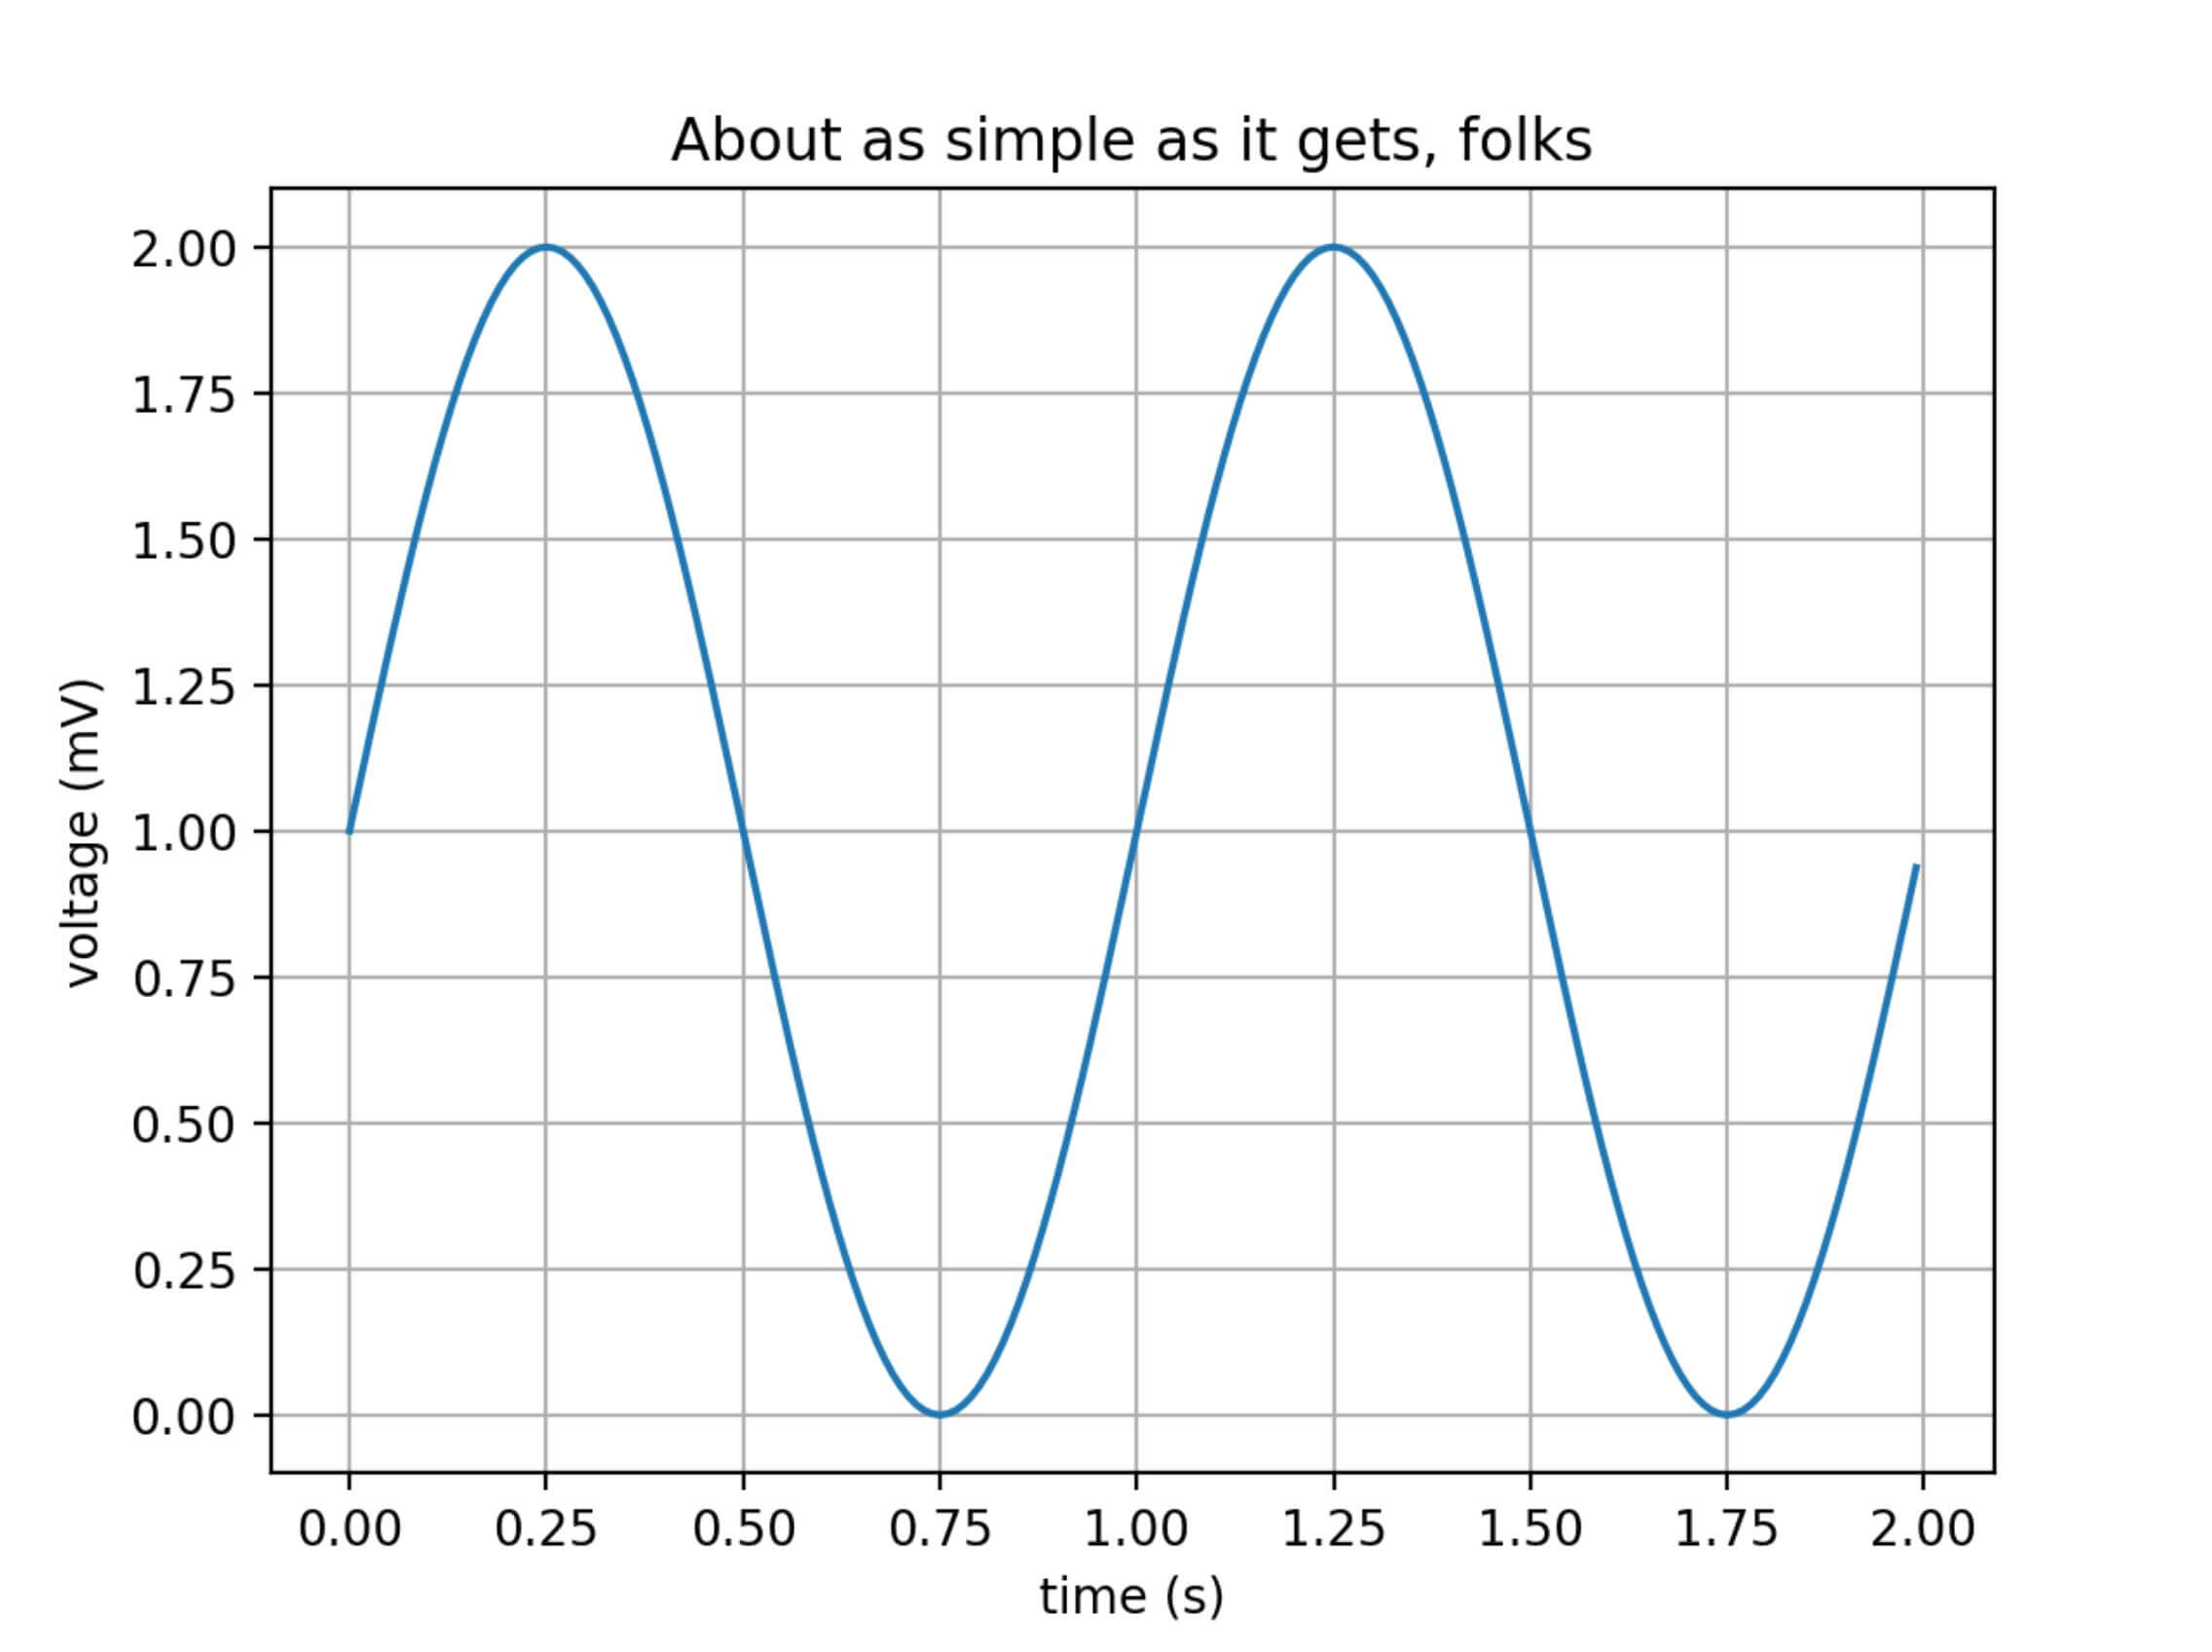
\includegraphics[width = 0.6\textwidth]{example1.jpg}
    \caption{Test Figure}
\end{figure}

\clearpage
\subsection{常用命令展示}
这部分将展示其他常用命令。

\begin{tbox}{颜色设置}
\begin{itemize}
	\item  \textcolor{Red}{赤}\textcolor{Orange}{橙}\textcolor{Yellow}{黄}\textcolor{Green}{绿}\textcolor{Emerald}{青}\textcolor{Blue}{蓝}\textcolor{Purple}{紫}
	\item  谁持彩练当空舞
\end{itemize}
\end{tbox}

\begin{tbox}{字号设置}
\begin{enumerate}
	\item {\LARGE 江晚正愁余}
	\item {\Large 江晚正愁余}
	\item {\large 江晚正愁余}
	\item {\normalsize 江晚正愁余}
	\item {\small 江晚正愁余}
	\item {\footnotesize 江晚正愁余}
	\item {\scriptsize 江晚正愁余}
\end{enumerate}
\end{tbox}

\begin{tbox}{字体设置(中文)}
\begin{enumerate}
	\item 宋体:{\songti 山有扶苏,隰有荷华}
	\item 仿宋:{\fangsong 山有扶苏,隰有荷华}
	\item 黑体:{\heiti 山有扶苏,隰有荷华}
	\item 楷书:{\kaishu 山有扶苏,隰有荷华}
\end{enumerate}
\end{tbox}

\begin{tbox}{Set font(English)}
\begin{enumerate}
	\item roman:\quad{\rmfamily Hello world!}
	\item sans-serif:\quad{\sffamily Hello world!}
	\item typewriter:\quad{\ttfamily Hello world!}
\end{enumerate}
\end{tbox}

\begin{tbox}{公式}
	无编号公式
    \begin{equation*}
        J(\theta) = \mathbb{E}_{\pi_\theta}[G_t] = \sum_{s\in\mathcal{S}} d^\pi (s)V^\pi(s)=\sum_{s\in\mathcal{S}} d^\pi(s)\sum_{a\in\mathcal{A}}\pi_\theta(a|s)Q^\pi(s,a)
    \end{equation*}
$$ J(\theta) = \mathbb{E}_{\pi_\theta}[G_t] = \sum_{s\in\mathcal{S}} d^\pi (s)V^\pi(s)=\sum_{s\in\mathcal{S}} d^\pi(s)\sum_{a\in\mathcal{A}}\pi_\theta(a|s)Q^\pi(s,a) $$
    有编号公式
    \begin{equation}
        J(\theta) = \mathbb{E}_{\pi_\theta}[G_t] = \sum_{s\in\mathcal{S}} d^\pi (s)V^\pi(s)=\sum_{s\in\mathcal{S}} d^\pi(s)\sum_{a\in\mathcal{A}}\pi_\theta(a|s)Q^\pi(s,a)
    \end{equation}
    \begin{equation}
        J(\theta) = \mathbb{E}_{\pi_\theta}[G_t] = \sum_{s\in\mathcal{S}} d^\pi (s)V^\pi(s)=\sum_{s\in\mathcal{S}} d^\pi(s)\sum_{a\in\mathcal{A}}\pi_\theta(a|s)Q^\pi(s,a)
    \end{equation}
	波尔文积分
    \[
    \begin{cases}
        \vspace{0.2cm}
        \displaystyle{\int_{0}^{\infty} \frac{\sin(x)}{x}\dd{x} = \frac{\pi}{2}}\\
        \vspace{0.2cm}
        \displaystyle{\int_{0}^{\infty} \frac{\sin(x)}{x} \frac{\sin(x/3)}{x/3}\dd{x} = \frac{\pi}{2}} \\
        \vspace{0.2cm}\cdot\cdot\cdot\\
        \vspace{0.2cm}
        \displaystyle{\int_{0}^{\infty} \frac{\sin(x)}{x} \frac{\sin(x/3)}{x/3} \cdot\cdot\cdot \frac{\sin(x/13)}{x/13}\dd{x} = \frac{\pi}{2}}\\
        \displaystyle{\int_{0}^{\infty} \frac{\sin(x)}{x} \frac{\sin(x/3)}{x/3} \cdot\cdot\cdot \frac{\sin(x/15)}{x/15}\dd{x} = \frac{467807924713440738696537864469}{935615849440640907310521750000}\pi}
    \end{cases}  
    \]
	多行对齐公式
	\begin{align*} 
		\hat{H}^{(2)} &= \frac{1}{2}\sum_{\alpha}\sum_{\beta}\int \dd[3]{x}\dd[3]{x'} \hat{\psi}^\dagger_\alpha(\vb{x})\hat{\psi}_\beta^\dagger(\vb{x}')\qty[\sum_{\vb{q}\neq 0} \frac{4\pi e^2}{q^2}\mathrm{e}^{i\vb{q}\cdot(\vb{x}-\vb{x}')}]\hat{\psi}_{\beta}(\vb{x}')\hat{\psi}_\alpha(\vb{x})\\[.2cm]
		&=\frac{1}{2V}\sum_{\vb{k}}\sum_{\vb{k}'}\sum_{\vb{q}\neq 0}\sum_{\alpha}\sum_{\beta}\qty(\frac{4\pi e^2}{q^2})\hat{C}_{\vb{k}+\vb{q},\alpha}^\dagger\hat{C}_{\vb{k}'-\vb{q},\beta}^\dagger\hat{C}_{\vb{k}'\beta}\hat{C}_{\vb{k}\alpha}. 
	\end{align*}
\end{tbox}

\begin{tbox}{引用}
	对公式的引用,如\cref{equ:test}
	\begin{equation}
        J(\theta) = \mathbb{E}_{\pi_\theta}[G_t] = \sum_{s\in\mathcal{S}} d^\pi (s)V^\pi(s)=\sum_{s\in\mathcal{S}} d^\pi(s)\sum_{a\in\mathcal{A}}\pi_\theta(a|s)Q^\pi(s,a)
		\label{equ:test}
    \end{equation}
	对图像的引用,如\cref{fig:test}
	\begin{figure}[H]
		\centering
		
\includegraphics[width=0.3\textwidth]{example.png}
		\caption{测试图片}
		\label{fig:test}
	\end{figure}
	对表格的引用,如\cref{tab:test}
	\begin{table}[H]
		\renewcommand\arraystretch{1.5}
		\caption{一个空表格}
		\begin{tabularx}{\textwidth}{|p{0.15\textwidth}|X|X|X|X|}
		\hline
		 &  &  &  &  \\    
		\hline
		 &  &  & &  \\    
		\hline
		\end{tabularx}
		\label{tab:test}
	\end{table}
\end{tbox}

\begin{tbox}{表格}
	tabular可以自己更改宽度
	\begin{table}[H]
		\renewcommand\arraystretch{1.7}
		\centering
		\caption{一个空表格}
		\begin{tabular}{|p{0.15\textwidth}|p{0.15\textwidth}|p{0.15\textwidth}|p{0.15\textwidth}|}
		\hline
		&   &  &  \\
		\hline
		 &   &  &  \\
		\hline    
		\end{tabular}
	\end{table}
	tabularx可以自适应宽度
	\begin{table}[H]
		\renewcommand\arraystretch{1.7}
		\centering
		\caption{一个空表格}
		\begin{tabularx}{\textwidth}{|p{0.2\textwidth}|X|X|X|X|X|X|}
			\hline
			& &  &  &  &  &  \\
			\hline
			 & &  &  &  &  &  \\
			\hline
		\end{tabularx}
	\end{table}
\end{tbox}

\begin{tbox}{TikZ 示例}
	TikZ 是 LaTeX 里实力极为强劲的一个绘图宏包(其文档说明高达1000多页),可以用于绘制复杂的矢量图形。

	% https://github.com/st--/annotate-equations?tab=readme-ov-file
	\vspace{1em}
	\begin{equation*}
		\eqnmarkbox[blue]{node1}{G_{\alpha\beta}(\vb{x},\vb{x}';t,t')} = -i \eqnmarkbox[red]{node2}{\bra{\psi_{H}^{0}}} 
		\eqnmarkbox[olive]{node4}{\hat{\mathsf{T}}}\qty[\hat{\psi}_{H\alpha}(\vb{x},t)\hat{\psi}_{H\beta}^\dagger(\vb{x}',t')]\eqnmarkbox[red]{node3}{\ket{\psi_H^{0}}}.
	\end{equation*}
	\annotate[yshift=0.5em]{left}{node1}{Green's function}
	\annotate[yshift=0.5em]{right}{node4}{time ordering operator}
	\annotatetwo[yshift=-1em]{below}{node2}{node3}{ground state}
	\vspace{1em}

	以及

	\vspace{3em}
	\begin{equation*}
		\mathcal{O}\big(
			(
			\eqnmarkbox[NavyBlue]{p1}{p}
			\eqnmarkbox[OliveGreen]{k1}{\kappa}^3  % note that we have the ^3 outside the \eqnmark/\tikzmarknode arguments
			)
			\eqnmarkbox[WildStrawberry]{T1}{T}
			+
			(
			\eqnmarkbox[NavyBlue]{p2}{p}  % tikz nodes need distinct names!
			\eqnmark[OliveGreen]{k2}{\kappa}
			)
			(
			\eqnmarkbox[WildStrawberry]{T2}{T}^2
			\tikzmarknode{Is}{|\mathcal{I}^*|}  % manual \tikzmarknode works, too
			\eqnmarkbox[Plum]{Nb}{N_b}
			\eqnmark[RoyalPurple]{M}{M}
			)
		\big)
	\end{equation*}
	\annotatetwo[yshift=1em]{above}{p1}{p2}{\# of nodes}
	\annotatetwo[yshift=-1em,xshift=0.2ex]{below}{T1}{T2}{\# of graphs in $\hat{\mathcal{G}}_T$}
	\annotatetwo[yshift=-2em]{below}{k1}{k2}{max.\ indegree in $\hat{\mathcal{G}}_T$}
	\annotate[yshift=3em]{above,left}{Is}{size of set of allowed interventions}
	\annotate[yshift=1em]{above}{Nb}{\# of samples per batch}
	\annotate[yshift=-1em]{below}{M}{\# of samples for $\mathbb{E}_y$}
	\vspace{3em}

	\begin{figure}[H]
		\centering
		\begin{tikzpicture}[
			pin edge={shorten <=5*\lrad},
			cross/.style={fill=white,path picture={\draw[black] (path picture bounding box.south east) -- (path picture bounding box.north west) (path picture bounding box.south west) -- (path picture bounding box.north east);}},
			dressed/.style={fill=white,postaction={pattern=north east lines}},
			momentum/.style 2 args={->,semithick,yshift=5pt,shorten >=5pt,shorten <=5pt},
			loop/.style 2 args={thick,decoration={markings,mark=at position {#1} with {\arrow{>},\node[anchor=\pgfdecoratedangle-90,font=\footnotesize,] {$p_{#2}$};}},postaction={decorate}}
		  ]
		  \def\lrad{1}
		  \def\mrad{0.175*\lrad}
		  \def\srad{0.15*\lrad}
		  \draw[loop/.list={{0.25}{1},{0.75}{2}}] (0,0) circle (\lrad);
		  \draw[cross] (-\lrad,0) circle (\srad) node[left=2pt] {$\partial_k R_{k,ij}(p_1,p_2)$};
		  \draw[dressed] (\lrad,0) circle (\mrad) node[right=2pt] {$\bigl[\Gamma_k^{(2)} + R_k\bigr]_{ji}^{-1}(p_2,p_1)$};
		\end{tikzpicture}
	\end{figure}
	\begin{figure}[H]
		\centering
		\subfloat[]{
			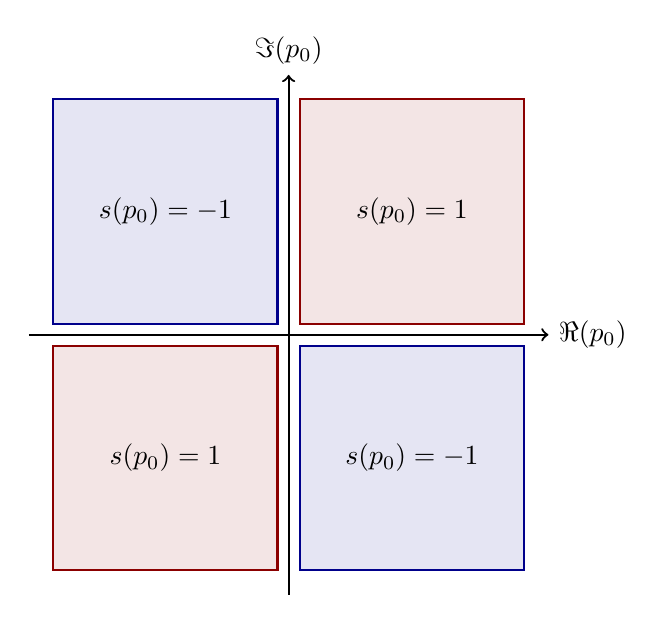
\begin{tikzpicture}[thick]
				\def\xr{3} \def\yr{3}
				% Axes
				\draw[->] (-\xr*1.1, 0) -- (\xr*1.1, 0) node [right] {$\Re(p_0)$};
				\draw[->] (0, -\yr*1.1) -- (0, \yr*1.1) node[above] {$\Im(p_0)$};
			  
				% Squares
				\draw[xshift=4, yshift=4, scale=0.95, DarkRed, fill=DarkRed!10] (0, 0) rectangle (\xr, \yr) node[black, midway] {$s(p_0) = 1$};
				\draw[xshift=-4, yshift=4, scale=0.95, DarkBlue, fill=DarkBlue!10] (0, 0) rectangle (-\xr, \yr) node[black, midway] {$s(p_0) = -1$};
				\draw[xshift=-4, yshift=-4, scale=0.95, DarkRed, fill=DarkRed!10] (0, 0) rectangle (-\xr, -\yr) node[black, midway] {$s(p_0) = 1$};
				\draw[xshift=4, yshift=-4, scale=0.95, DarkBlue, fill=DarkBlue!10] (0, 0) rectangle (\xr, -\yr) node[black, midway] {$s(p_0) = -1$};
			\end{tikzpicture}
		}
		\subfloat[]{
			\begin{tikzpicture}[>={Kite[inset=0pt,length=0.32cm,bend]},
				decoration={markings,
				mark= at position .2 with {\arrow{>}},
				mark= at position .4 with {\arrow{>}},
				mark= at position .65 with {\arrow{>}},
				}
			]
				\def\gap{0.3}
				\def\bigradius{3}
				\def\littleradius{0.5}
				\def\gapp{2}
			
				% contour
			\filldraw[postaction = {decorate}, thick ,fill=gray!40] 
			let 
				\n1 = {asin(\gap/2/\bigradius)},
				\n2 = {asin(\gap/2/\littleradius)},
				\n3 = {\littleradius* cos(\n2)}
			in
				(0+\n1:\bigradius) node[above right]{$R$} (\gapp - \n3,\gap/2) arc(180-\n2:\n2:\littleradius) -- (\n1:\bigradius)
				 arc (0+\n1:360-\n1:\bigradius) -- (\gapp + \n3,-\gap/2) arc(-\n2:-180+\n2:\littleradius)--
				 (0-\n2:\littleradius) arc (360-\n2:0+\n2:\littleradius) node[above right]{$\delta$} -- cycle;
			
				\draw[thick,->] (300:\littleradius) arc (300:130:\littleradius) node[above]{$C_{\delta}$};
				\draw[thick,->] ([xshift=2cm] 300:\littleradius) arc (300:270:\littleradius) node[below]{$C_{\delta_1}$};
				\draw[thick,->] ([xshift=2cm] 120:\littleradius) arc (120:80:\littleradius) node[above]{$C_{\delta_2}$};
			
				\fill (\gapp,0) circle(2.5pt);
				\node at (50:\bigradius+0.3){$C_{R}$};
				% axes
				\draw[-Latex] (-1.2*\bigradius,0) -- (1.2*\bigradius,0) node[below]{$\Re$} ;
				\draw[-Latex] (0,-1.2*\bigradius) -- (0,1.2*\bigradius) node[right]{$\Im$};
			\end{tikzpicture}
		}
	\end{figure}
	\begin{figure}[H]
		\centering
		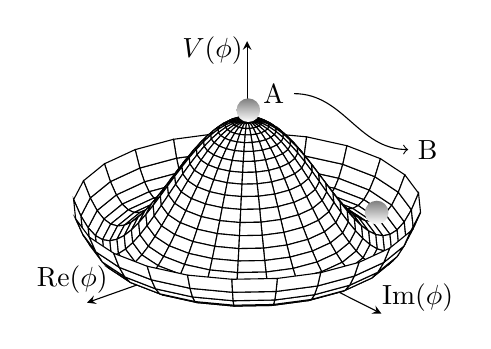
\begin{tikzpicture}
			\pgfplotsset{compat=1.8}
			\begin{axis}[
				axis lines=center,
				view={140}{25},
				axis equal,
				domain=0:360,
				y domain=0:1.25,
				xmax=1.5,ymax=1.5,zmin=0,zmax=1.5,
				x label style={at={(axis description cs:0.18,0.29)},anchor=north},
				y label style={at={(axis description cs:0.82,0.25)},anchor=north},
				z label style={at={(axis description cs:0.44,0.8)},anchor=north},
				xlabel = $\mathrm{Re}(\phi)$,
				ylabel=$\mathrm{Im}(\phi)$,
				zlabel=$V(\phi)$,
				ticks=none,
				clip bounding box=upper bound
			  ]
		  
			  \addplot3 [surf, shader=flat, draw=black, fill=white, z buffer=sort] ({sin(x)*y}, {cos(x)*y}, {(y^2-1)^2});
			\end{axis}
			\shade (3.47,3.5) circle [radius=0.15cm];
			\shade (5.1,2.2) circle [radius=0.15cm];
			\node[anchor=east] at (4.05,3.71) (text) {A};
			\node[anchor=west] at (5.5,3.0) (description) {B};
			\draw (description) edge[out=180,in=0,<-] (text);
		  \end{tikzpicture}
	\end{figure}

	\begin{figure}[H]
		\centering
		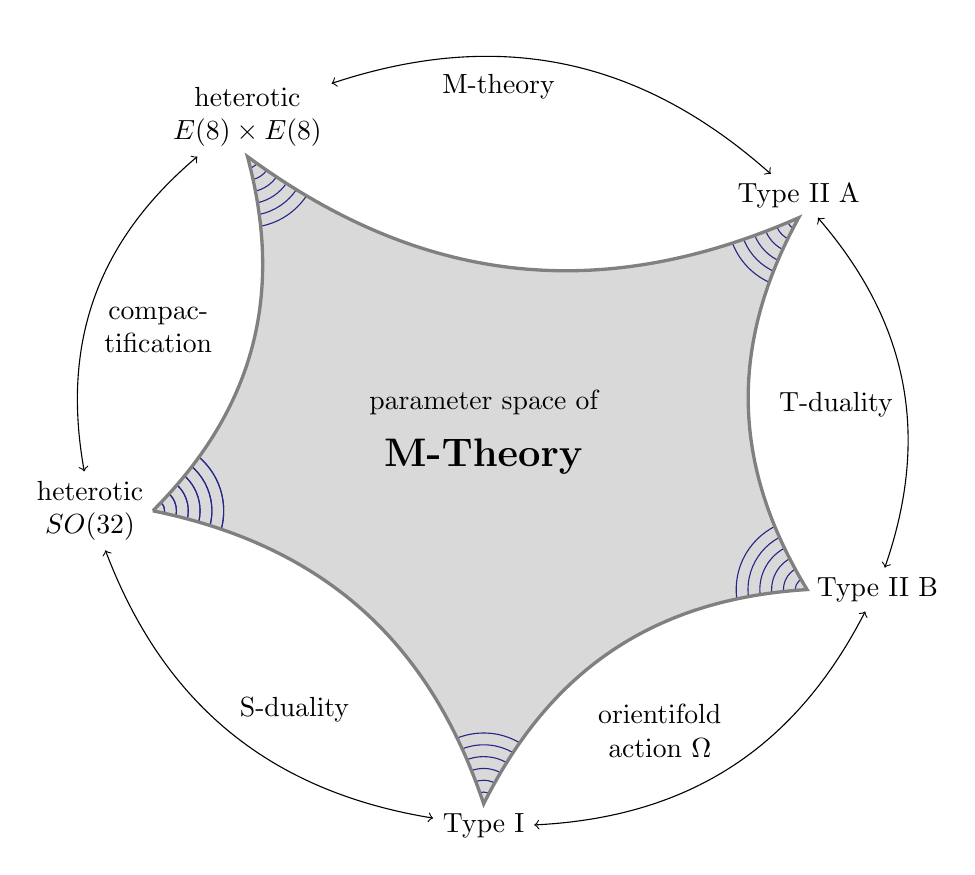
\begin{tikzpicture}

			\node (so32) [align=center] at (-5,-1) {heterotic\\$SO(32)$};
			\node (e8e8) [align=center] at (-3,4) {heterotic\\$E(8) \times E(8)$};
			\node (tiia) [align=center] at (4,3) {Type II A};
			\node (tiib) [align=center] at (5,-2) {Type II B};
			\node (ti) [align=center] at (0,-5) {Type I};
		  
			\draw[bend left,<->] (so32) to node [below right,align=center] {compac-\\tification} (e8e8);
			\draw[bend left,<->] (e8e8) to node [below left] {M-theory} (tiia);
			\draw[bend left,<->] (tiia) to node [below left] {T-duality} (tiib);
			\draw[bend left,<->] (tiib) to node [above left,align=center] {orientifold\\action $\Omega$} (ti);
			\draw[bend left,<->] (ti) to node [above right] {S-duality} (so32);
		  
			\begin{scope}
			  \clip[bend right]
			  (so32.east)
			  to (e8e8.south)
			  to (tiia.south)
			  to (tiib.west)
			  to (ti.north)
			  to (so32.east);
			  \foreach \c in {so32.east,e8e8.south,tiia.south,tiib.west,ti.north,so32.east}{%
				  \foreach \r in {1,...,6}{%
					  \draw[DarkBlue] (\c) circle (\r*0.15cm);
					}
				}
			\end{scope}
		  
			\draw[bend right,very thick,gray,fill,fill opacity=0.3] (so32.east) to (e8e8.south) to (tiia.south) to (tiib.west) to (ti.north) to (so32.east);
		  
			\node (mth) [align=center] at (0,0) {parameter space of\\[2ex]{\Large \textbf{M-Theory}}};
		  
		  \end{tikzpicture}
	\end{figure}

	\begin{figure}[H]
		\centering
		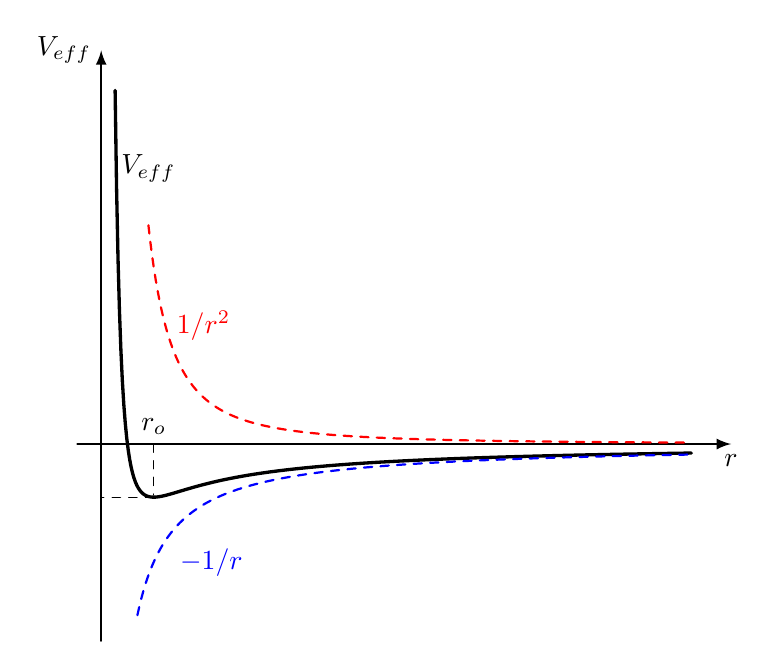
\begin{tikzpicture}[line cap=round]
			% Axis
			\draw[thick, -latex] (-2ex,0) -- (8,0) node[below] {$r$};
			\draw[thick, -latex] (0,-2.5) -- (0,5) node[left] {$V_\text{eff}$};	
			
			% Plot Function
			\draw[domain=0.177:7.5, samples=400, variable=\r, very thick] plot ({\r},{0.3/(\r*\r)-0.9/\r});
			\draw[domain=0.6:7.5, samples=300, variable=\r, thick, dashed, red] plot ({\r},{1/(\r*\r)});
			\draw[domain=0.46:7.5, samples=300, variable=\r, thick, dashed, blue] plot ({\r},{-1/(\r)});
			
			% Dashed
			\draw[dashed] (2/3,0) -- +(0,-0.65) node[pos=0, above] {$r_o$};
			\draw[dashed] (2/3,-0.68) -- (0,-0.68);		
			
			% Nodes
			\node at (0.6,3.5) {$V_\text{eff}$};
			\node[red] at (1.3,1.5) {$1/r^2$};
			\node[blue] at (1.4,-1.5) {$-1/r$};
		\end{tikzpicture}
	\end{figure}

\end{tbox}
\end{document}
